\begin{frame}
    \frametitle{Lab CPU}
    \begin{itemize}
        \item Port-Mapped I/O
        \item First 256 addresses are reserved for I/O
        \item Special instructions for I/O (IN, OUT)
        \item I/O devices are connected to the CPU through the bus
        \item CPU is pooling the I/O devices
        \item Status and Command registers for each device are mapped to the same I/O addresses
        \item Data registers are mapped to the next I/O addresses
        \item Can be changed to memory-mapped I/O or DMA
    \end{itemize}
\end{frame}

\begin{frame}
    \frametitle{Lab I/O}
    \begin{figure}
        \centering
        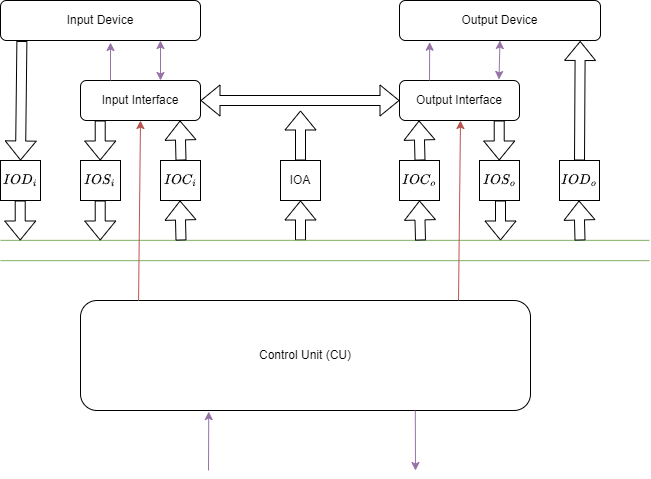
\includegraphics[width=0.8\textwidth]{media/io.png}
    \end{figure}
\end{frame}

\begin{frame}
    \frametitle{Lab I/O DMA}
    \begin{itemize}
        \item 8 registers for DMA into the I/O space (let's start from 0x08)
    \end{itemize}
    \begin{table}[]
        \resizebox{\textwidth}{!}{%
            \begin{tabular}{|c|c|c|}
                \hline
                \textbf{Address} & \textbf{Name} & \textbf{Function} \\ \hline
                0x08 & SCIO0 & Status/Command Register for IO device 0 \\ \hline
                0x09 & SCIO1 & Status/Command Register for IO device 1 \\ \hline
                0x0a & SCIO2 & Status/Command Register for IO device 2 \\ \hline
                0x0b & SCIO3 & Status/Command Register for IO device 3 \\ \hline
                0x0c & SCDMA & Status/Command Register for DMA \\ \hline
                0x0d & MADMA & Memory Address Register for DMA \\ \hline
                0x0e & CNTDMA & Count Register for DMA \\ \hline
                0x0f & INITDMA & Initialize DMA Register \\ \hline
            \end{tabular}
        }
    \end{table}
\end{frame}

\begin{frame}
    \frametitle{Architecture with DMA}
    \begin{figure}
        \centering
        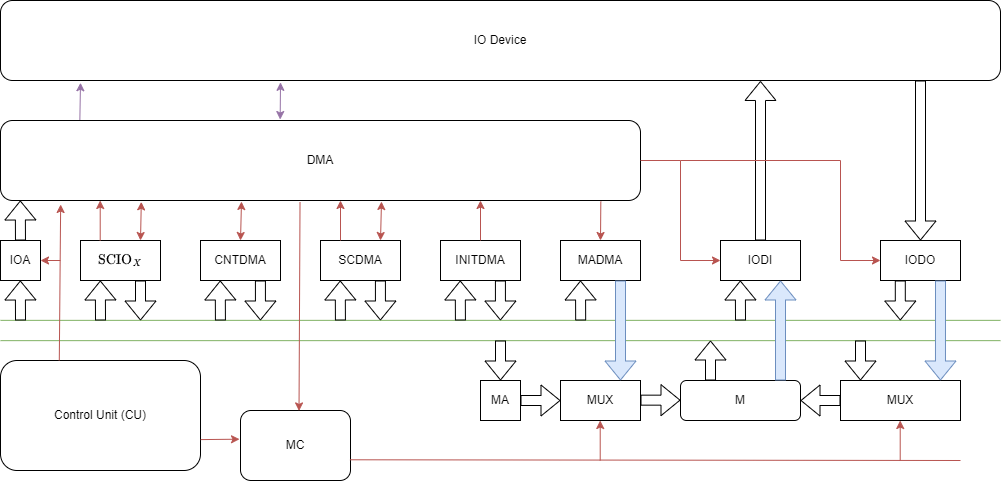
\includegraphics[width=0.9\textwidth]{media/dma.png}
    \end{figure}
\end{frame}

\begin{frame}
    \frametitle{SCDMA Register}
    \begin{table}[]
        \resizebox{\textwidth}{!}{%
            \begin{tabular}{|c|c|c|c|c|c|c|c|c|c|c|c|c|c|c|c|c|}
                \hline
                \textbf{0} & \textbf{1} & \textbf{2} & \textbf{3} & \textbf{4} & \textbf{5} & \textbf{6} & \textbf{7} & \textbf{8} & \textbf{9} & \textbf{10} & \textbf{11} & \textbf{12} & \textbf{13} & \textbf{14} & \textbf{15} \\ \hline
                $SIO_{0}$ & $SIO_{1}$ & $SIO_{2}$ & $SIO_{3}$ & X & X & SDMA & EOBT & EXTIRQ & X & PIRQ & ENIRQ & X & MT & DT & ENT \\ \hline
            \end{tabular}
        }
    \end{table}
    \begin{itemize}
        \item $SIO_{0-3}$ - Status of the I/O devices 0 - functional 1 - not functional
        \item SDMA - DMA is active for 0 - inactive for 1
        \item EOBT - End of block transfer for 0 - not for 1
        \item EXTIRQ - There is an external interrupt from IO device for 0 - not for 1
        \item PIRQ - There is a programable interrupt from CPU for 0 - not for 1 (testing)
        \item ENIRQ - Enable interrupt for 0 - disable for 1
        \item MT - Mode of transfer 0 - block for 1 - cycle stealing
        \item DT - Direction of transfer 0 - from IO to memory to IO for 1 - from memory to IO
        \item ENT - Enable transfer for 0 - disable for 1
    \end{itemize}
    \note{
    }
\end{frame}

% \begin{frame}
%     \frametitle{Exam Question}
%     Template: Having the following IO registers value, main memory address and data, what can you find on the data bus?

%     Example: Having the following IO registers value, main memory address and data, what can you find on the data bus?
%     \begin{columns}
%         \column{0.5\textwidth}
%     \begin{table}[]
%         \begin{tabular}{|l|l|}
%             \hline
%             \textbf{Register} & \textbf{Value} \\ \hline
%             SCDMA & 0x1234 \\ \hline
%             MADMA & 0x5678 \\ \hline
%             CNTDMA & 0x0001 \\ \hline
%             INITDMA & 0x0002 \\ \hline
%             SCIO0 & 0x0000 \\ \hline
%             SCIO1 & 0x0000 \\ \hline
%             SCIO2 & 0x0000 \\ \hline
%             SCIO3 & 0x0000 \\ \hline
%         \end{tabular}
%     \end{table}
%     \column{0.5\textwidth}
%     \begin{table}[]
%         \begin{tabular}{|l|l|}
%             \hline
%             \textbf{Memory Address} & \textbf{Data} \\ \hline
%             0x5678 & 0x0000 \\ \hline
%             0x5679 & 0x0001 \\ \hline
%             0x567a & 0x0002 \\ \hline
%             0x567b & 0x0003 \\ \hline
%             0x567c & 0x0004 \\ \hline
%             0x567d & 0x0005 \\ \hline
%             0x567e & 0x0006 \\ \hline
%             0x567f & 0x0007 \\ \hline
%         \end{tabular}
%     \end{table}
%     \end{columns}

% \end{frame}
